

Is it possible to harvest energy from water without moving parts?
What is the electrical impedance between electrodes in an electrolyte solution?
These questions form the basis of this thesis.
Although seemingly unrelated, the answer to both lies in behaviour occurring wherever liquid comes into contact with a solid.
That behaviour is the formation of arranged layers of liquid against the solid surface, called a double layer.
This thesis is separated into two parts; each addressing one of the two questions related to double layers.
\Cref{part:doubleLayersOnInsulators} studies double layers on insulating solids as a means of energy conversion.
Methods using these layers as a means of power harvesting are trialled and measured.
A particular application of such a harvester is discussed and its feasibility assessed.
\Cref{part:doubleLayersOnConductors} models the electrical impedance between two electrodes when submerged in an electrolyte.
Double layers play a large role this impedance as they dictate the concentration of ions electrode's surface.
Measurement of interface impedance allows for direct comparison between a range of environments into which electrodes are placed.
This is important when designing an implant that will be placed inside a person.
Before introducing background material on interfacial double layers, my motivation for doing this work is discussed.
This is followed by a statement of originality and an outline of the structure of this thesis.


\section{Motivation}


  My thesis began with the question ``is it possible to harvest energy from water without moving parts?''
  The purpose for such a harvester is to power an electronic water meter.
  Doing this without the moving parts of more traditional mechanisms, such as turbines, should increase the harvester's life expectancy and be generally more robust.
  I started by looking at three possible harvesting mechanisms;
  \begin{itemize}
    \item piezoelectric vibrators
    \item electrostatic generators
    \item streaming potential cells
  \end{itemize}
  The piezoelectric vibrator was the equivalent of a water whistle with a vibrational energy harvester attached; the electrostatic generator was a version of Lord Kelvin's Electrostatic Generator with a harvesting application; and the streaming potential cell was a mystery.
  We knew geologists used streaming potentials to measure underground water flow.
  The only thing we knew about the mechanism was that forcing water through something somehow generated a voltage.
  Learning about that mechanism and answering the following questions started me on the path that became this thesis.
  \begin{enumerate}
    \item Where does streaming voltage come from?
    \item What role does the geometry of a streaming device play?
    \item Could you change the materials to get more voltage?
  \end{enumerate}
  After experimentation and energy budgeting, I eventually concluded that streaming cell harvesters are not yet practical.
  Low conversion efficiency, a susceptibility to clogging and the need for high manufacturing tolerances make them unsuited for domestic water metering.
  However, this research allowed me to gain  a working knowledge of interfacial double layers.

  During my doctoral studies my supervisor, Jonathan Scott, took a sabbatical at Saluda Medical in Sydney.
  At the time, Saluda were developing a medical implant for spinal stimulation.
  Jonathan and Saluda's senior electronic engineer developed an electrical model of the impedance presented by electrodes immersed in a solution of saline.
  That model uses electrical components to simulate the electrical impedance between an electrode and an electrolyte.
  This means it can be entered into electrical simulation software and used to simulate an implanted electrode.
  Much of the behaviour the model simulates is due to double layers.
  Saluda's engineers use a dilute solution of phosphate buffered saline to approximate human spinal cavities; into which their electrodes are implanted.
  They do not know how good this approximation is, it was the most appropriate mixture they had.
  The alternative is to embed an electrode in a live animal and measure the response - that is also what they do.
  Live animal experiments are costly and how they differ from solutions of saline is unknown.
  The interface model is the starting point for the second phase of my research; characterising the interface between an electrode and biological solutions.
  I leveraged my understanding of interfacial double layers to understand how the model worked, and use it correctly.


\section{Statement of Originality}


  Measurements of the energy consumed during an EEPROM write, an ADC measurement, a single instruction being executed, and during sleep mode for six 8-bit microprocessors are my own.
  The relationship between an electrolyte's conductivity and the impedance of the constant phase element, presented in~\Cref{part:doubleLayersOnConductors}, is my own.
  The recipe for a mixture that improves the match between live sheep spine and test solutions such as phosphate buffered saline is my own.
  The method of measuring faradaic current that removes the effect of double layer capacitance between electrodes in an electrolyte is my own.


\section{Publications arising from this work}


  \begin{itemize}
    \item Jones, M.H. \& Scott, J. (2014). \emph{Scaling of Electrode-Electrolyte Interface Model Parameters In Phosphate Buffered Saline.} Published in IEEE Transactions on Biomedical Circuits and Systems, Issue 99.
    \item Jones, M.H. \& Scott, J. (2014). \emph{Feasibility of Harvesting Power to Run a Domestic Water Meter Using Streaming Cell Technology.} In proceedings of the 21st Electronics New Zealand Conference, ENZCON 2014, Waikato University, Hamilton, New Zealand.
    \item Jones, M.H. \& Scott, J.B. (2011). \emph{The energy efficiency of 8-bit low-power microcontrollers.} In Proceedings of the 18th Electronics New Zealand Conference, ENZCON 2011, Massey University, Palmerston North, 21-22 November 2011, pp. 87-90.
  \end{itemize}

\section{Thesis Outline}

  This thesis is broken into two parts.
  Part~\ref{part:doubleLayersOnInsulators} is concerned with the concept of using double layers to harvest energy.
  This relates to the streaming cell energy harvester.
  Part~\ref{part:doubleLayersOnConductors} involves the electrode-electrolyte interface model put forward by Jonathan Scott to investigate the behaviour of double layers on electrodes.
  Put simply, Part~\ref{part:doubleLayersOnInsulators} deals with double layers on insulating surfaces, and Part~\ref{part:doubleLayersOnConductors} deals with double layers on conductive surfaces.

  The first chapter of part~\ref{part:doubleLayersOnInsulators} (\cref{chap:harvesterIntroduction}) begins with background on streaming cells, followed by a review of related literature.
  Then in \cref{chap:harvestingEnergy}, I build and measure the electrical output of ten streaming cells.
  This is used to determine the energy conversion efficiency of streaming cells fabricated using readily available methods.
  Next, \cref{chap:wirelessWaterMetering} looks into the possibility of using a streaming cell harvester to power an electronic water meter.
  The quantity of harvestable energy is estimated by modelling the water consumption in a typical New Zealand home.
  \Cref{chap:energyRequirements} looks at the components of an electronic water meter and estimates the amount of energy they are likely to need.
  Bringing these estimates and measurements together, \cref{chap:part_1_discussion} discusses the feasibility of energy harvesting using streaming cells.
  Finally, in \cref{chap:part_1_conclusion}, the work done in \cref{part:doubleLayersOnInsulators} is summarised and concluding comments are made on the findings.


\section{Background}


  Modelling and measuring the electrical aspects of interfacial double layers draws on both electronic and chemical concepts.
  Those with an electronic background are unlikely to be familiar with double layers.
  This section provides background on what a double layer is and how it forms.
  It begins by discussing liquids and moves toward defining the double layer itself.


  \subsection{Liquid}
  
    % Liquid
    \begin{figure}
        \begin{center}
            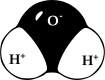
\includegraphics{content/introduction/graphics/polarWater}
        \end{center}
        \caption{Molecular model of a water molecule}
        \label{fig:waterMolecule}
    \end{figure}
    A double layer is an organised layer of liquid; two layers to be precise.
    Its formation is the response of material in the liquid phase responding to charge trapped in a solid phase.
    Because double layers are a property of liquids it is important to put liquid itself into perspective.
    At the macroscopic scale, individual atoms and molecules liquids interact with massive complexity.
    The density of atoms and molecules in a liquid at the microscopic scale is extreme.
    Water, the most abundant liquid on earth, is formed from polar molecules.
    This means that one side appears to be negatively charged, while the other appears positively charged.
    \Cref{fig:waterMolecule} shows the molecule in the form of a molecular diagram, notice its broken symmetry along the horizontal plane.
    This separation of charge in space is responsible for complex behaviour.
    An electric field causes water molecules to rotate, or polarise, so as to align itself within the field.
    A body of water, or any polar liquid, responds to electric fields and the presence of charge.

    % Interfaces
    \begin{figure}[h]
        \begin{center}
            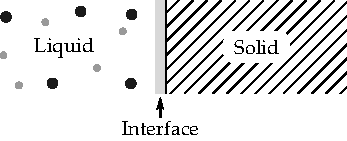
\includegraphics{content/introduction/graphics/simpleLayerDiagram}
        \end{center}
        \caption{Diagram showing the location of the fluid-solid interface}
        \label{fig:interfaceDiagram}
    \end{figure}
    The boundary between any two states of matter is referred to as an interface; it is simply where two things meet.
    We are interested specifically in the dynamics of the solid-liquid interface.
    Interactions relevant to double layers occur in a thin region inside the liquid at the interface.
    When there is a difference in charge between the solid surface and the liquid bulk, a double layer forms.
    The following three statements are capture underlying nature of double layers.
    \begin{itemize}
      \item The charged elements in a solid are fixed in place, but in a liquid they are free to move.
      \item Any charge imbalance between solid and liquid will be greatest at the point they meet.
      \item Charges interact with each other, whether by repulsion or attraction.
    \end{itemize}
    The consequence being that any charge interactions will be most pronounced within the liquid phase at the surface of the solid.

    % Shielding
    \begin{figure}
        \begin{center}
            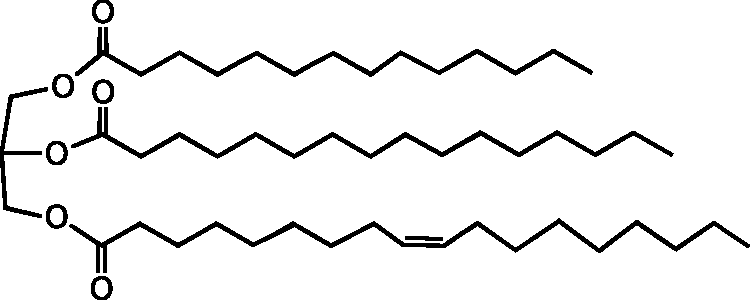
\includegraphics[scale=0.8]{content/introduction/graphics/butterfat}
        \end{center}
        \caption{Structural formula of a butterfat molecule}
        \label{fig:butterfat}
    \end{figure}
    A solid solid may refer to the walls of a container or particulates suspended in solution.
    When a particulate is suspended throughout a solution it is referred to as an emulsion.
    For example, milk is such an emulsion of butterfat in water.
    \Cref{fig:butterfat} shows the structure of a butterfat molecule; a long structure that behaves as a solid.
    The stability of an emulsion, such as milk, depends on the strength of the double layers that encapsulate each particle.
    These double layers shield the molecules or particles from one another electrically.
    By shielding them from each other they are unable to collect and bond together.
    This shielding prevents milk from coagulating and turning to lumps.
    Having addressed where double layers come from, as well as their organisation, the anatomy of these layers is now introduced.


  \subsection{Interfacial double layers}


    \begin{figure}
      \begin{center}
        
\includegraphics{content/introduction/graphics/counterAndCoIons}
      \end{center}
      \caption{Counter-ions are oppositely charged, co-ions have like charge.}
      \label{fig:counterAndCoIons}
    \end{figure}
    In the previous section, a brief explanation of what a double layer is and where they form was introduced.
    We next look at double layer anatomy and define some of its properties.
    Before moving on, use of the terms `co-ion' and `counter-ion' is defined.
    These terms refer to ions containing charge -- like or opposite -- in polarity to a second charge or body of charge.
    For example, if a negatively charged surface attracts positively charged ions then positive ions are the counter-ion.
    Likewise, if a positively charged surface was to repel a positive ion then the positive ion is the co-ion.
    The terms are convenient because they remove the need to identify specific polarities in discussion.
    This relationship is shown in~\cref{fig:counterAndCoIons}.


    \subsubsection*{Models of the interfacial double layer}


      \begin{figure}
        \begin{center}
          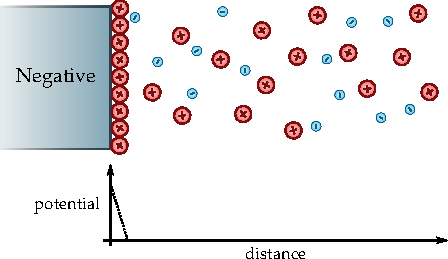
\includegraphics{content/introduction/graphics/model_helmholtz}
        \end{center}
        \caption{Structure of the Helmholtz layer.}
        \label{fig:doubleLayerModel_helmholtz}
      \end{figure}
      Three models of the interfacial double layer have been proposed over time.
      Each represents an extension or modification of the previous, beginning with the Helmholtz Model~\cite{Horch2004}.
      Helmholtz proposed his parallel plate capacitor based model in 1879~\cite{Geddes1997}.
      His model consists of two layers of surface charge, one inside the solid and one in the liquid.
      The counter-ions sit in a \emph{compact layer}, meaning that they are bound to the surface and immobile.~\cite{Salieb-Beugelaar2009}
      Figure \ref{fig:doubleLayerModel_helmholtz} represents this as a row of tightly packed positive ions along the solid surface.
      Past the layer of bound surface ions there is no affect from the solid's charged surface.
      In essence, his model defines the interface a single layer of ions held against the edge of a solid.
      The problem with this model is its inability to predict the layer's capacitance.
      Measurement of a double layer's electrical capacitance changes depending on either the electrical potential across the layer, or the concentration of ions in the solution~\cite{Bard1980}.
      The Stern model does not account for this variation.
      
      \begin{figure}
        \begin{center}
          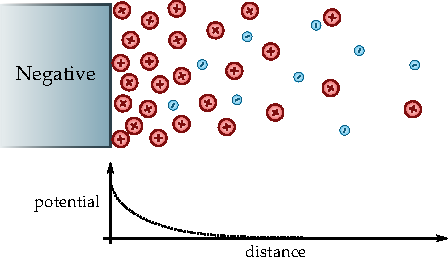
\includegraphics{content/introduction/graphics/model_guoyChapman}
        \end{center}
        \caption{Structure of the Goüy-Chapman layer.}
        \label{fig:doubleLayerModel_gouyChapman}
      \end{figure}
      Later, Goüy and Chapman independently proposed that charge in the liquid phase may instead be held in a \emph{diffuse layer}~\cite{Chapman1913}.
      This meant that ions in the layer were not fixed and that the density of charge in the layer could vary.
      Figure~\ref{fig:doubleLayerModel_gouyChapman} illustrates the concept by the lack of ions bound to the surface and the gradual decline in counter-ion concentration with distance from the surface.
      The Goüy-Chapmam Model accounts for the observed variation in capacitance by distributing charge in the liquid as a gradient from the surface of the solid.
      The layer is free to change its concentration profile in response to applied electrostatic potential and ionic concentration.
      In the case of a higher electrostatic potential, the layer is pulled closer to the surface, becoming shallower.
      In the case of a higher electrolytic concentration, the layer is more concentrated with a higher charge density, again becoming shallower.
      It predicts the change in capacitance by growing or shrinking the size of the layer, but it still fails to predict the capacitance at high ionic concentrations.
      This is in part because it fails to account for the physical size of the ions in the electrolyte and instead models them as point charges~\cite{Bard1980}.
      In their model, ions can get infinitely close to the surface regardless of their size.
      This becomes a problem at high ionic concentration where the surface becomes crowded.

      \begin{figure}
        \begin{center}
          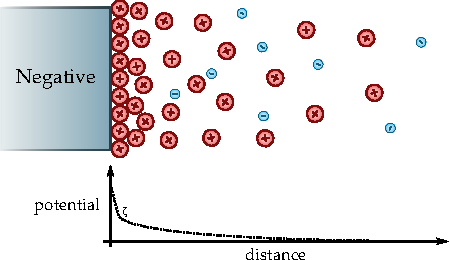
\includegraphics{content/introduction/graphics/model_stern}
        \end{center}
        \caption{Structure of the Goüy-Chapman-Stern layer.}
        \label{fig:doubleLayerModel_stern}
      \end{figure}
      In 1924, Otto Stern published his modified version of the Goüy-Chapmam model~\cite{Stern1924}.
      This model, illustrated in figure~\ref{fig:doubleLayerModel_stern} extends the Goüy-Chapmam model by setting the minimum distance an ion can get to the solid surface.
      This effectively reintroduces the compact layer as seen in Helmholtz's model but allows for a concentration gradient exterior to this layer.
      It resembles the Helmholtz model at high ionic concentration but accounts for spread in the layer dimensions at lower concentrations.
      The Stern, sometimes referred to as the Goüy-Chapmam-Stern, model is a well accepted double layer model~\cite{Olthuis2005}.


    \subsubsection*{Anatomy of an interfacial double layer}


      \begin{figure}
        \begin{center}
          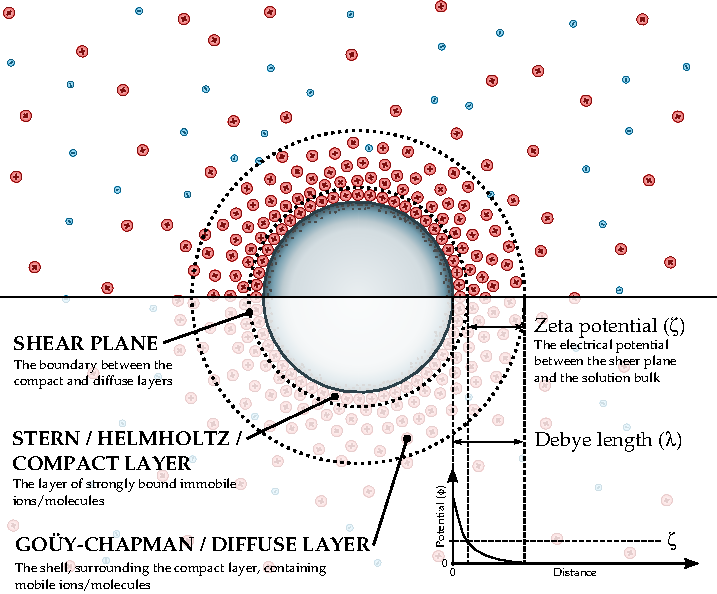
\includegraphics{content/introduction/graphics/doubleLayer_version2}
        \end{center}
        \caption{Anatomy of the double layer}
        \label{fig:doubleLayer_anatomy}
      \end{figure}
      Figure~\ref{fig:doubleLayer_anatomy} shows the double layer organisation according to the currently accepted Goüy-Chapmam-Stern model.
      It shows the compact layer adsorbed to the surface of the suspended solid.
      In this layer the ions are immobile due to the electrical strength at the surface.
      Surrounding this layer is the diffuse layer.
      Ions here are still drawn to the solid, but not so strongly as to be immobile.
      The electric potential in this layer decays from that within the compact layer to the potential in the bulk of the solution.
      These layers are divided by the shear plane.
      The shear plane represents nearest distance from the surface at which the layer can move laterally.
      This is an important parameter with linear geometries, such as the inside of a pipe, as it represents the true no-slip boundary.
      The thickness of a typical double layer is between \SI{1}-\SI{100}{\nano\meter}~\cite{Jiang2010}, as defined by its Debye length~\cite{Israelachvili2011}.
      The Debye length is the distance between the interface and the point in the liquid where the electric potential is no longer affected by the charged interface.
      As mentioned in the previous section, this varies based on the ionic concentration of the solution and the potential at the solid surface.


  % Marcus Wilson tore this apart, don't even mention computer simulation.
  %\subsection{Liquid simulation}
    %\label{sub:molecularSimulation}


    %At the macroscopic scale, liquid behaviour is simple and calculable.
    %Modern computers can simulate the movement of liquids using the Navier-Stokes equations with accuracy and speed.
    %Engineers simulate the flow of liquids, or any Newtonian fluid, routinely using computer design tools.
    %These tools allow engineers to push boundaries of aircraft and boat design.
    %However, this does not hold true when modelling fluid at the microscopic scale due to the required scale. 
    %%Computer simulations are  based upon calculating the state of a system of objects at specific time intervals.
    %%There are other methods, such as 
    %%At each computed time interval the variables of each element of a system are updated and the cycle repeats.
    %%This repeats for every time-step until the simulation time-frame has run its course.
    %%These simulations are not run in real-time; instead taking hours or days to compute simulations spanning fractions of a second.

%%    Finite-difference time-domain simulation is a common technique for calculating electrical fields and resulting currents and voltages in the field of electrical engineering.
%%    Such simulations can involve hundreds of thousands, \emph{sometimes millions}, of objects.
%%    These objects are elements of a 3D mesh created to represent the geometry of the system.
%%    Because of the dependence on neighbouring parameter values, each time-step may take many passes over each element in a system to calculate the final state before moving on.
%%    This type of simulation is common whenever the effects of radio waves need to be simulated.

    %Designing and conditioning computer simulations at a molecular scale are challenging.
    %Simulating the interface is possible, but is very involved and constitutes a field of its own.
    %The work of Nagy et al.\ ~\cite{Nagy1992} and Bazant et al.\ ~\cite{Bazant2011} has shed light on some of the underlying physical mechanics of the double layer.
    %Matters are complicated by the fact that some aspects of the double layer are still not fully understood~\cite{Kornyshev2007}.

    %Simulation of a liquid having a sensible macroscopic volume is impractical.
    %The molar mass of water is \SI{18.0528}{\gram\per\mole}.
    %One gram of water is defined as one millilitre, so we can say that for every millilitre of water we have we have an eighteenth of a mole of water.
    %Avagadro's constant, the number of constituent particles per mole of a given substance, is $6.0221\thinspace \times 10^{23}$.
    %Therefore we have one eighteenth of Avagadro's constant in water molecules, which is about $3.3333\times 10^{22}$ molecules.
    %Molecular simulation has not been employed here.
    %Useful results are likely to be obtained from volumes less than \SI{1}{\milli\litre}, but the time and resources to successfully run and validate such simulations are high.
    %Such simulations are shaping the underlying models of the interfacial double layer~\cite{Kornyshev2007}.

